% igs2ejournalguide.tex
% v4.00 3-sept-2015

\NeedsTeXFormat{LaTeX2e}

% check that the math fits the two-column format:
 \documentclass[twocolumn, letterpaper]{igs}

% but use this version when submitting your article:
 % \documentclass[review,oneside, letterpaper]{igs}

 % \usepackage{igsnatbib}
  \usepackage{lmodern}
\usepackage{amsmath,amssymb,amsthm}
\usepackage{natbib} 
\usepackage{wrapfig}
\usepackage{enumitem}
\usepackage{multirow}
\usepackage{tabularx}
\usepackage{booktabs}

% check if we are compiling under latex or pdflatex
  \ifx\pdftexversion\undefined
    \usepackage[dvips]{graphicx}
  \else
    \usepackage[pdftex]{graphicx}
    \usepackage{epstopdf}
    \epstopdfsetup{suffix=}
  \fi


\begin{document}

\title[]{Analysis of methods and uncertainties in estimating winter surface mass balance from direct measurements on alpine glaciers}

\author[]{Alexandra PULWICKI,$^1$
  Gwenn E. FLOWERS,$^1$ Valentina  RADI\'C,$^2$}

\affiliation{%
$^1$ Simon Fraser University, Burnaby, BC, Canada\\
$^2$University of British Columbia, Vancouver, BC, Canada\\
  Correspondence: Alexandra Pulwicki 
  $<$apulwick@sfu.ca$>$}


%%%%%%%%%%%%%%%%%%%%%%%%%%%%%%%%%
%	ABSTRACT
%%%%%%%%%%%%%%%%%%%%%%%%%%%%%%%%%

\abstract{Accurately estimating winter surface mass balance for a glacier is central to quantifying overall mass balance and melt runoff. However, measuring and modelling snow distribution and variability is inherently difficult in alpine terrain, resulting in high mass balance uncertainty. The goal of this paper is to provide a comprehensive sweep of choices and assumptions present when moving from snow observations to winter mass balance estimates and to better understand how interactions between snow variability, data error and our methodological choices contribute to uncertainty. We extensively measure snow depth and density, at various spatial scales, on three glaciers in the St. Elias Mountains, Yukon. Elevation is found to be the dominant driver of accumulation variability but the relationship varies between glaciers. Our results also suggest that wind redistribution and preferential deposition affect snow distribution but that more complex parametrization is need to fully capture wind effects. We use a Monte Carlo method to quantify the effects of variability due to density interpolation method, snow water equivalent observations as well as observation interpolation on estimates of winter surface mass balance. The largest source of uncertainty stems from calculating parameters for interpolation using either linear regression or simple kriging. Spatially extensive measurements in the accumulation area are needed, at the expense of detailed ablation area measurements, to better constrain interpolation models and reduce uncertainty.  }

\maketitle




%%%%%%%%%%%%%%%%%%%%%%%%%%%%%%%%%
%	INTRODUCTION
%%%%%%%%%%%%%%%%%%%%%%%%%%%%%%%%%
\section{Introduction}

Accurate estimation of winter surface mass balance is critical for correctly simulating the summer and overall mass balance of a glacier \citep{Reveillet2016}. Effectively representing spatial distribution of snow is also important for simulating snow and ice melt as well as energy and mass exchange between the land and atmosphere to better monitor surface runoff and its downstream effects \citep{Clark2011}. Snow distribution is sensitive to a number of complex process that partially depend on glacier location, topography, and orientation \citep{Bloschl1991, Mott2008, Clark2011, Sold2013}. Current models are not able to fully represent these processes so the distribution of snow in remote, mountainous locations is not well known. There is, therefore, a significant source of uncertainty that undermines the ability of models to represent current glacier conditions and make predictions of glacier response to a warming climate \citep{Reveillet2016}. 

Winter mass balance is the sum of accumulation and ablation over the winter season \citep{Cogley2011}, and constitutes the addition of glacier mass when considering the net mass balance. In this study, we attempt to estimate winter surface mass balance, which is the net accumulation and ablation assuming no internal snow pack accumulation in the form of ice lenses \citep{Cogley2011}. We refer to this quantity as winter balance, defined as the change of mass during a winter season, throughout the paper. Accurate estimates of winter balance are critical for mass balance estimates, not only because winter balance constitutes half of the mass balance but also because the distribution of snow on a glacier initializes the summer balance and high snow albedo contributes to reduced summer melt \citep{Hock2005,Reveillet2016}. Winter balance is typically measured at a few stake locations and interpolation methods are the same as those of summer balance \citep[e.g.][]{Hock1999, MacDougall2011, Cullen2017}. This equivalence is likely inappropriate because snow distribution is largely driven by precipitation \citep{Lehning2008} and wind patterns\citep{Bernhardt2009,Musselman2015}, which are known to be highly heterogeneous in alpine environments \citep{Barry1992}. Snow distribution is therefore highly variable and has short correlation length scales \citep[e.g.][]{Anderton2004, Egli2011, Grunewald2010, Helbig2017, Lopez2011, Lopez2013, Machguth2006, Marshall2006}. Melt is strongly affected by air temperature and solar radiation \citep{Hock2005}, both of which are consistent across large spatial domains \citep{Barry1992}. Further, detailed studies of winter balance are far less common than those of summer balance and uncertainty in winter mass balance currently overshadows differences between summer balance models \citep{Reveillet2016}. It is therefore necessary to investigate methods that address the variability of snow distribution and will improve estimates and decrease uncertainty of winter balance. 

Winter balance is notoriously difficult to estimate. Snow distribution in alpine regions is highly variable and influenced by dynamic interactions between the atmosphere and complex topography operating on multiple spatial and temporal scales \citep{Barry1992, Liston2006, Clark2011}. Extensive, high resolution and accurate accumulation measurements on glaciers are almost impossible to achieve due to cost benefits of the various methods used to quantify snow water equivalent \citep{Cogley2011, McGrath2015}. For example, snow probes obtain accurate point observations but have negligible spatial coverage. Conversely, gravimetric methods obtain extensive measurements of mass change but cannot capture relevant spatial variability of snow \citep{Cogley2011}. Glacierized regions are also generally remote and challenging to access during the winter due to poor travelling conditions. 

Predicting winter balance is a further challenge. Physically-based dynamic models are able to capture the intricate interactions between the atmosphere and local topography but they are operationally complex and computationally expensive, and require a diverse set of detailed observations \citep[e.g.][]{Mott2008, Dadic2010}. Empirical models that rely on statistical relationships between proxy parameters and measured accumulation are widely applied and simple to execute but most are unable to explain the majority of variance observed or lack insight into processes that affect snow distribution \citep[e.g.][]{Grabiec2011,Lopez2011}.

There is currently a disparity in snow survey sophistication within mass balance studies when compared to snow science studies. Studies that aim to estimate the end-of-winter, basin-wide snow water equivalent (SWE) within the snow science literature employ a wide range of snow measurement techniques, including direct measurement \citep[e.g.][]{Elder1991}, lidar/photogrammerty \citep[e.g.][]{Deems2006, Nolan2015} and ground penetrating radar\citep[e.g.][]{Godio2016}. Surveys are designed to measure snow throughout the basin and ensure that all terrain types are sampled. A wide array of measurement interpolation methods are used, including linear \citep[e.g.][]{Lopez2010} and non-linear regressions \citep[e.g.][]{Molotch2005}and geospatial interpolation \citep[e.g.][]{Erxleben2002}such as kriging, and methods are often combined to yield improved fit \citep[e.g.][]{Balk2000}. Physical snow models, such as Alpine3D \citep{Lehning2006} and SnowDrift3D \citep{Schneiderbauer2011}, are continuously being improved and tested within the snow science literature. Snow survey error has been considered from both a theoretical \citep{Trujillo2015} and applied perspective \citep{Turcan1975,Woo1978, Deems2006}. 

Winter mass balance surveys employ similar techniques and methods, favouring more basic approaches \citep{Kaser2003, Sold2013}. Measurement tools overlap between snow science and glaciology but spatial coverage is often limited for winter balance studies and typically consist of an elevation transect along the glacier centreline \citep[e.g.][]{Kaser2003, Machguth2006}. Interpolation of these measurements is primarily done by computing a linear regression that includes only a few topographic parameters \citep[e.g.][]{MacDougall2011}, with elevation being the most common. Other applied techniques include hand contouring \citep[e.g.][]{Tangborn1975}, kriging \citep[e.g.][]{Hock1999} and attributing measured accumulation values to elevation bands. Physical snow models have been applied on a few glaciers \citep{Mott2008, Dadic2010} but a lack of detailed meteorological data generally prohibits their wide-spread application. Error analysis is rarely considered and to our knowledge, no studies have investigated uncertainty in winter balance estimates. By investigating tools and methodologies applied in snow science literature, we hope to identify ways to improve snow survey design and estimates of SWE.

There is clearly a need for more comprehensive understanding of uncertainties inherent when estimating accumulation on glaciers. Ultimately, we need a thorough knowledge of the processes that affect spatial and temporal snow variability and an effective method to predict snow accumulation. The contribution of our work toward these goal is to (1) examine methods and uncertainties when moving from snow measurements to estimating winter balance and (2) show how snow variability, data error and our methodological choices interact to create uncertainty in our estimate of winter balance. We focus on commonly applied low-complexity methods of measuring and predicting winter balance with the hope of making our results broadly applicable to current and future winter mass balance programs.


%%%%%%%%%%%%%%%%%%%%%%%%%%%%%%%%%
%	STUDY SITE
%%%%%%%%%%%%%%%%%%%%%%%%%%%%%%%%%

\section{Study site}

Winter balance surveys were conducted on three glaciers in the Donjek Range of the St. Elias Mountains, located in the south western Yukon, Canada. The Donjek Range is approximately $30\times30$ km and Glacier 4, Glacier 2, and Glacier 13 (labelling adopted from \cite{Crompton2016}) are located along a SW-NE transect through the range. There is a local topographic divide in the Donjek Range that follows an ``L'' shape, with one glacier located in each of the south, north, and east regions (Figure \ref{fig:Sampling}). These mid-sized alpine glaciers are generally oriented SE-NW, with Glacier 4 dominantly south facing and Glaciers 2 and 13 generally north facing. The glaciers are low angled with steep head walls and steep valley walls. The St. Elias mountains boarder the Pacific Ocean and rise sharply, creating a significant climatic winter gradient between coastal maritime conditions, generated by Aleutian--Gulf of Alaska low-pressure systems, and interior continental conditions, determined by Yukon--Mackenzie high-pressure system \citep{Taylor1969}. The average dividing line between the two climatic zones shifts between Divide Station and the head of the Kaskawalsh Glacier based on synoptic conditions. The Donjek Range is located approximately 40 km to the east of the head of the Kaskawalsh Glacier. Research on snow distribution and glacier mass balance in the St. Elias is limited. A series of research programs were operational in the 1960s \citep{Wood1948, Danby2003} and long-term studies on a few alpine glaciers have arisen in the last 30 years \citep[e.g.][]{Clarke1984, Paoli2009}.

\begin{table}[]
\centering
\caption{Physical details of study glaciers}
\label{tab:GlacierDetails}
\begin{tabular}{cccccc}
\hline
\textbf{} & \multirow{2}{*}{\textbf{Location}} & \multicolumn{2}{c}{\textbf{Elevation (m a.s.l)}} & \textbf{Slope ($^{\circ}$)} & \multirow{2}{*}{\textbf{\begin{tabular}[c]{@{}c@{}}Area\\ (km)\end{tabular}}} \\
 &  & \textit{Mean} & \textit{Range} & \textit{Mean} &  \\ \hline
\textbf{G4} & \begin{tabular}[c]{@{}c@{}}595470 E\\ 6740730 N\end{tabular} & 2344 & 1958--2809 & 12.8 & 3.8 \\
\textbf{G2} & \begin{tabular}[c]{@{}c@{}}601160 E\\ 6753785 N\end{tabular} & 2495 & 1899--3103 & 13.0 & 7.0 \\
\textbf{G13} & \begin{tabular}[c]{@{}c@{}}604602 E\\ 6763400 N\end{tabular} & 2428 & 1923--3067 & 13.4 & 12.6
\end{tabular}
\end{table}

%%%%%%%%%%%%%%%%%%%%%%%%%%%%%%%%%
%	METHODS
%%%%%%%%%%%%%%%%%%%%%%%%%%%%%%%%%


\section{Methods}

Estimating winter balance involves transforming snow depth and density measurements to distributed estimates of snow water equivalent (SWE). We use four main processing steps. First, we obtain measurements of snow depth and density. Since density is measured more sparsely than depth, the second step is to interpolate density measurements to all depth measurement locations and to calculate the SWE at each measurement location. Third, we average all SWE values within one grid cell of a digital elevation model (DEM) with given spatial resolution to produce a single value of SWE for each grid cell. Fourth, we interpolate SWE values to obtain a distributed estimate of SWE across the surface of the glacier. We choose to use a linear regression between SWE and topographic parameters as well as simple kriging to interpolation grid cell SWE. To estimate the specific winter balance we then calculate aerially-averaged integrated SWE. For brevity, we refer to these four steps as (1) field measurements, (2) distributed snow density, (3) grid cell average SWE and (4) distributed SWE. Detailed methodology for each step is outlined below.

\subsection{Field measurements}

\begin{figure*}
	\centering
	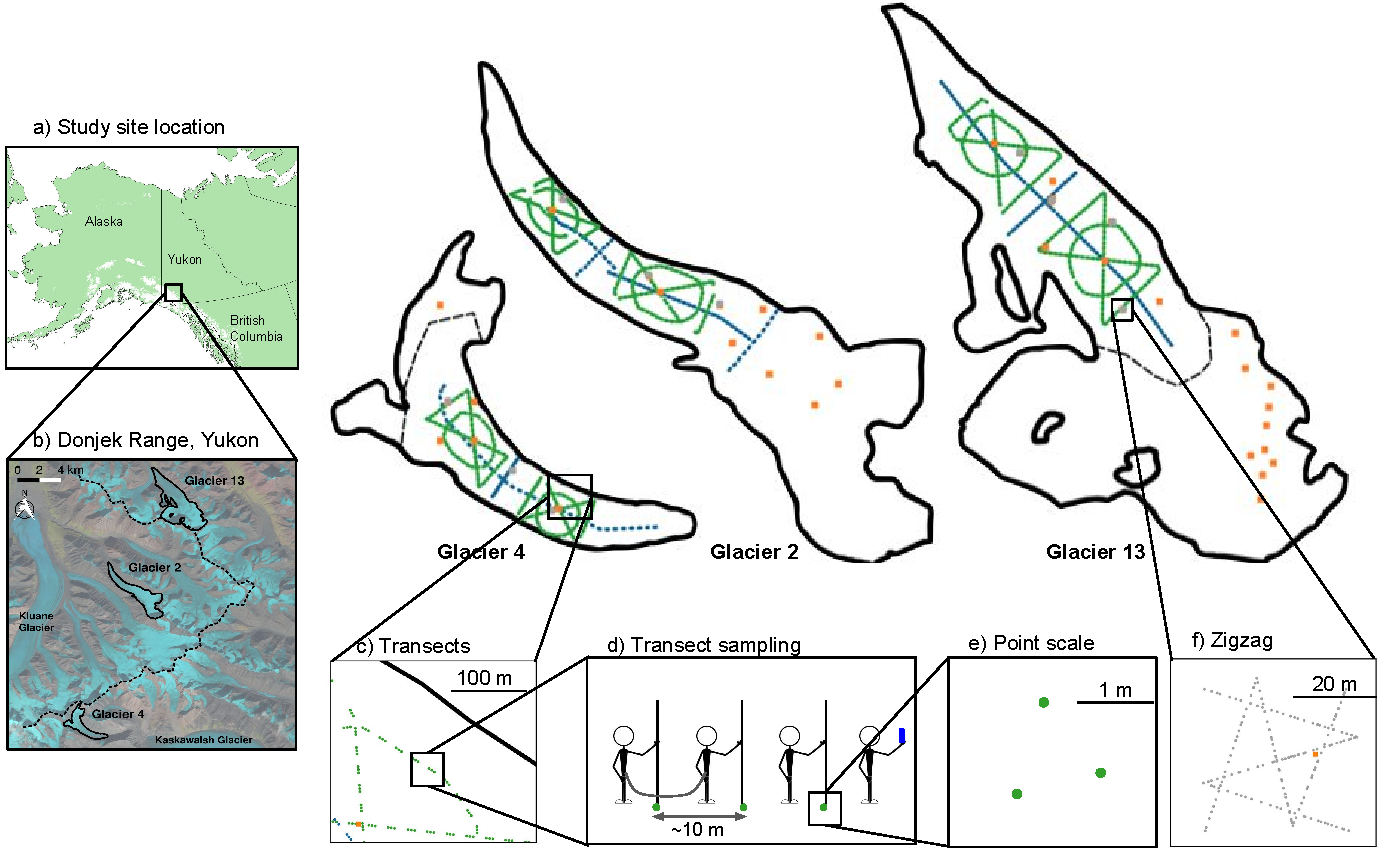
\includegraphics[width =\textwidth]{Sampling.pdf}\\
	\caption{Sampling design for Glaciers 4, 2 and 13, located in the Donjek Range, Yukon (a,b). Centreline and transverse transects are shown in blue dots, hourglass and circle design are shown in green dots. (c) Linear and curvilinear transects typically consist of sets of three measurement locations, spaced $\sim$10 m apart (d). (e) At each measurement location, three snow depth observation are made. (f) Linear-random snow depth measurements in `zigzag' design are shown as grey dots. Orange squares are locations of snow density measurements. }
	\label{fig:Sampling}
\end{figure*}

\begin{table}[]
\centering
\caption{Details of snow survey conducted in May 2016 at Glacier 4 (G4), Glacier 2 (G2), and Glacier 13 (G13). Values shown include number of snow depth measurement locations along transects ($n_{T}$), total length of transects ($d_T$ [km]), number of combined SP and FS density measurement locations ($n_{\rho}$) and number of zigzag ($n_{zz}$). }
\label{tab:SurveyDetails}
\begin{tabular}{cccccc}
\hline
\textbf{} & \textbf{Date} & \textbf{$n_{T}$} & \textbf{$d_T$} & \textbf{$n_{\rho}$} & \textbf{$n_{zz}$} \\ \hline
\textbf{G4} & May 4--7 & 649 & 13.1 & 7 & 3 \\
\textbf{G2} & May 8--11 & 762 & 13.6 & 7 & 3 \\
\textbf{G13} & May 12--15 & 941 & 18.1 & 19 & 4
\end{tabular}
\end{table}

\subsubsection{Sampling design}

The sampling design attempted to capture depth variability at multiple spatial scales. We measured winter balance at three glaciers along the precipitation gradient in the St. Elias Mountains, Yukon \citep{Taylor1969} in an attempt to account for range-scale variability \citep{Clark2011}. We measured winter balance on Glaciers 4, 2, and 13, which are located increasingly far from the head of the Kaskawalsh Glacier (Figure \ref{fig:Sampling}b). Snow depth was measured along linear and curvilinear transects to account for basin-scale variability. At each measurement location, three values of snow depth were recorded to account for point-scale variability \citep{Clark2011}.  We selected centreline and transverse transects with sample spacing of $10-60$ m (Figure \ref{fig:Sampling}d) to capture previously established correlations between elevation and accumulation \citep[e.g.][]{Machguth2006, Walmsley2015} as well as accumulation differences between ice-marginal and centre accumulation. We also implemented an hourglass and circle design (Figure \ref{fig:Sampling}), which allows for sampling in all directions and easy travel (Parr, C., 2016 personal communication). At each measurement location, we took $3-4$ depth measurements within $\sim$1 m of each other (Figure \ref{fig:Sampling}e), resulting in more than 9,000 snow depth measurements throughout the study area. 

\subsubsection{Snow depth}

The estimated SWE is the product of the snow depth and depth-averaged density. Snow depth is generally accepted to be more variable than density \citep{Elder1991, Clark2011, Lopez2013} so we chose a sampling design with relatively small measurement spacing along transects that resulted in a ratio of approximately 55:1 snow depth to snow density measurements. Our sampling campaign involved four people and occurred between May 5 and 15, 2015, which corresponds to the historical peak accumulation in the Yukon (Yukon Snow Survey Bulletin and Water Supply Forecast, May 1, 2016). While roped-up for glacier travel at fixed distances between observers, the lead person used a single frequency GPS (Garmin GPSMAP 64s) to navigate as close to the predefined transect measurement locations as possible (Figure \ref{fig:Sampling}). The remaining three people used 3.2 m aluminium avalanche probes to take snow depth measurements. The location of each set of depth measurements, taken by the second, third and fourth observers, was approximated based on the recorded location of the first person. 

Snow depth sampling was primarily done in the ablation area to ensure that only snow from the current accumulation season was measured. Determining the boundary between snow and firn in the accumulation area, especially when using an avalanche probe, is difficult and often incorrect \citep{Grunewald2010,Sold2013}. We intended to use a firn corer to extract snow cores in the accumulation area but due to environmental conditions we were unable to obtain cohesive cores. Successful measurements within the accumulation area were done either in a snow pit or using a Federal Sampler with shovel validation so that we could identify the snow-firn transition based on a change in snow crystal size and density. 

\subsubsection{Zigzags}

To capture variability at spatial scales smaller than a DEM grid cell, we implemented a linear-random sampling design, termed `zigzag' \citep{Shea2010}. We measured depth at random intervals ($0.3 - 3.0$ m) along two `Z'-shaped transects within three to four $40\times40$ m squares (Figure \ref{fig:Sampling}c) resulting in $135-191$ measurement points for each zigzag. Zigzag locations were randomly chosen within the upper ($\sim$2350 m a.s.l.), middle ($\sim$2250 m a.s.l.), and lower portions ($\sim$2150 m a.s.l.) of the ablation area of each glacier. We were able to measure a fourth zigzag on Glacier 13 that was located in the middle ablation area ($\sim$2200 m a.s.l.).

\subsubsection{Snow density}

Snow density was measured using a wedge cutter in three snowpits on each glacier. We measured a vertical density profile by inserting a $5\times10\times 10$ cm wedge-shaped cutter (250 cm$^3$) in 5 cm increments to extract snow samples and then weighed the samples with a spring scale \citep[e.g.][]{Gray1981,Fierz2009}. Uncertainty in estimating density from snow pits stems from measurement errors and incorrect assignment of density to layers that could not be sampled (i.e. ice lenses and `hard' layers). 

While snow pits provide the most accurate measure of snow density, digging and sampling a snow pit is time and labour intensive. Therefore, a Federal Snow Sampler (FS) \citep{Clyde1932}, which measures bulk SWE, was used to augment the spatial extent of density measurements. A minimum of three measurements were taken at each of $7-19$ locations on each glacier and an additional eight FS measurements were co-located with each snow pit profile. Measurements where the snow core length inside the FS was less than 90\% of the snow depth were assumed to be an incorrect sample and were excluded. Density values were then averaged for each location. 

During the field campaign there were two small accumulation events. The first, on May 6, also involved high winds so accumulation could not be determined. The second, on May 10, resulted in 0.01 m w.e accumulation at one location on Glacier 2. Warm temperatures and clear skies occurred between May 11 and 16, which we believed resulted in significant melt occurring on Glacier 13. The snow in the lower part of the ablation area was isothermal and showed clear signs of melt and snow metamorphosis. The total amount of accumulation and melt during the study period could not be estimated so no corrections were made. 

\subsection{Distributed snow density}

Measured density is interpolated to estimate SWE at each depth sampling location. We chose four separate methods that are commonly applied to interpolate density: (1) mean density over an entire range \citep[e.g.][]{Cullen2017}, (2) mean density for each glacier \citep[e.g.][]{Elder1991, McGrath2015}, (3) linear regression of density with elevation \citep[e.g.][]{Elder1998, Molotch2005} and (4) inverse-distance weighted density \citep[e.g.][]{Molotch2005}.  SP and FS densities are treated separately, for reasons explained below, which results in eight density interpolation options. 

\subsection{Grid cell average SWE}

We average SWE values within each DEM-aligned grid cell. The locations of measurements have considerable uncertainty both from the error of the GPS unit ($2.7 - 4.6$ m) and the estimation of observer location based on the GPS unit. These errors could easily result in the incorrect assignment of a SWE measurement to a certain grid cell but this source of variability was not further investigated because we assume that SWE variability is captured in the zigzag measurements described below. There are no significant differences between observers (p$>$0.05), with the exception of the first transect on Glacier 4. No corrections to the data based on observer differences are applied.

\subsection{Distributed SWE}

\subsubsection{Linear regression}

SWE are interpolated and extrapolated for each glacier using linear regression (LR) as well as simple kriging (SK). Linear regressions relate observed SWE to grid cell values of DEM-derived topographic parameters \citep{Davis1986}. We choose to include elevation, distance from centreline, slope, aspect, curvature, ``northness'' and a wind redistribution parameter in the LR. Topographic parameters are weighted by a set of fitted regression coefficients ($\beta_i$). Regression coefficients are calculated by minimizing the sum of squares of the vertical deviations of each data point from the regression line \citep{Davis1986}. The distributed estimate of SWE is found by using regression coefficients to estimate SWE at each grid cell. Specific winter balance is calculated as the aerially-averaged, integrated SWE for each glacier ([m w.e.]). 

Snow depth data are highly variable so there is a possibility for the LR to fit to this data noise, a process known as overfitting. To prevent overfitting, cross-validation and model averaging are implemented. First, cross-validation is used to obtain a set of $\beta_i$ values that have greater predictive ability. We select 1000 random subsets (2/3 values) of the data to fit the LR and the remaining data (1/3 values) are used to calculate a root mean squared error (RMSE) \citep{Kohavi1995}. Regression coefficients resulting in the lowest RMSE are selected. Second, we use model averaging to take into account uncertainty when selecting predictors and to also maximize predictive ability \citep{Madigan1994}. Models are generated by calculating a set of $\beta_i$ for all possible combinations of predictors. Following a Bayesian framework, model averaging involves weighting all models by their posterior model probabilities \citep{Raftery1997}. To obtain the final regression coefficients, the $\beta_i$ values from each model are weighted according to the relative predictive success of the model, as assessed by the Bayesian Information Criterion (BIC) value \citep{Burnham2004}. BIC penalizes more complex models, which further reduces the risk of overfitting.

\subsubsection{Topographic parameters}

Topographic parameters are easy to calculate proxies for physical processes, such as orographic precipitation, solar radiation effects, wind redistribution and preferential deposition. We derive all parameters for our study from a SPOT-5 DEM ($40\times40$ m) \citep{Korona2009}. Elevation ($z$) values were taken from the SPOT-5 DEM directly. Distance from centreline ($d_C$) was calculated as the minimum distance between the Easting and Northing of the northwest corner of each grid cell and a manually defined centreline. Slope, aspect and curvature were calculated using the \texttt{r.slope.aspect} module in GRASS GIS software run through QGIS as described in \cite{Mitavsova1993} and \cite{Hofierka2009}. Slope ($m$) is defined as the angle between a plane tangential to the surface (gradient) and the horizontal \citep{Olaya2009}. Aspect ($\alpha$) is the dip direction of the slope and $\sin(\alpha)$, a linear quantity describing a slope as north/south facing, is used in the regression. Mean curvature ($\kappa$) is found by taking the average of profile and tangential curvature. Profile curvature is the curvature in the direction of the surface gradient and it describes the change in slope angle. Tangential curvature represents the curvature in the direction of the contour tangent. Curvature differentiates between mean-concave (positive values) terrain with relative accumulation and mean-convex (negative values) terrain with relative scouring \citep{Olaya2009}. ``Northness'' ($N$) is defined as the product of the cosine of aspect and sine of slope \citep{Molotch2005}. A value of $-1$ represents a vertical, south facing slope, a value of $+1$ represents a vertical, north facing slope, and a flat surface yields 0. The wind exposure/shelter parameter (Sx) is based on selecting a cell within a certain angle and distance from the cell of interest that has the greatest upward slope relative to the cell of interest \citep{Winstral2002}. Sx was calculated using an executable obtained from Adam Winstral that follows the procedure outlined in \cite{Winstral2002}. 

Visual inspection of the curvature fields calculated using the DEM showed a noisy spatial
distribution that did not vary smoothly. To minimize the effect of noise on parameters sensitive to DEM grid cell size, we applied a $7\times7$ grid cell smoothing window to the DEM, which was then used to calculate curvature, slope, aspect and ``northness''.

\subsubsection{Simple kriging}

Simple kriging (SK) estimates SWE values at unsampled locations by using the isotropic spatial correlation (covariance) of measured SWE to find a set of optimal weights \citep{Davis1986, Li2008}. SK assumes that if sampling points are distributed throughout a surface, the degree of spatial correlation of the observed surface can be determined and the surface can then be interpolated between sampling points. We used the \texttt{DiceKriging} R package \citep{Roustant2012} to calculate the maximum likelihood covariance matrix, as well as range distance ($\theta$) and nugget. The range distance is a measure of data correlation length and the nugget is the residual that encompasses sampling-error variance as well as the spatial variance at distances less than the minimum sample spacing \citep{Li2008}. 

\subsection{Quantifying effects of uncertainty}

We identify three major sources of uncertainty within the process of translating snow measurements to winter balance. These uncertainty sources encompass error and uncertainty within each processing step. When calculating distributed density, the density interpolation method is the largest source of uncertainty. We therefore carry all density interpolation options forward in the estimation of winter balance. When calculating a grid cell average SWE, uncertainty stems from a distribution of SWE values within each grid cell, which is assumed to be caused by random effects that are unbiased and unpredictable \citep{Watson2006}. We therefore choose to characterize SWE uncertainty by generating a normal distribution of SWE values for each measured grid cell. The normal distribution has a mean equal to the grid cell average SWE and a standard deviation equal to the mean standard deviation of all zigzags on each glacier. When obtaining interpolated SWE, the best fit interpolation itself has uncertainty based on the data that are used to fit the regression line or kriging surface. LR uncertainty is represented by obtaining a multivariate normal distribution of possible $\beta_i$ values. The standard deviation of each distribution is calculated using the covariance of regression coefficients as outlined in \cite{Bagos2015}. SK uncertainty is calculated using the \texttt{DiceKriging} package and is returned as an upper and lower 95\% confidence interval for SWE at each grid cell. We refer to the three uncertainty sources as (1) density uncertainty, (2) SWE uncertainty and (3) interpolation uncertainty. 

To quantify the effects of the three uncertainty sources on the final winter balance estimate, we conduct a Monte Carlo experiment, which uses repeated random sampling to calculate a numerical solution \citep{Metropolis1949}. In our study, we randomly sample the distributions for SWE uncertainty and interpolation uncertainty and carry these values through the data processing steps to obtain a value of winter balance. First, random values from the distribution of SWE values for each grid cell are independently chosen. Then, LR or SK is used to interpolate these SWE values. With the LR, a set of $\beta_i$ values and their distributions are calculated and the $\beta_i$ distributions are randomly sampled. These new $\beta_i$ values are used to calculate winter balance. With SK, a distribution of winter balance is calculated from the 95\% confidence interval kriging surfaces. Density uncertainty is accounted for by repeating the process for each density interpolation method. This random sampling process is done 1000 times, which results in a distribution of possible winter balance values based on uncertainty within the data processing steps.

%%%%%%%%%%%%%%%%%%%%%%%%%%%%%%%%%%%%%%%%%%%
%%  RESULTS 
%%%%%%%%%%%%%%%%%%%%%%%%%%%%%%%%%%%%%%%%%%%
\section{Results}

\subsection{Measurements}

\begin{figure*}
	\centering
	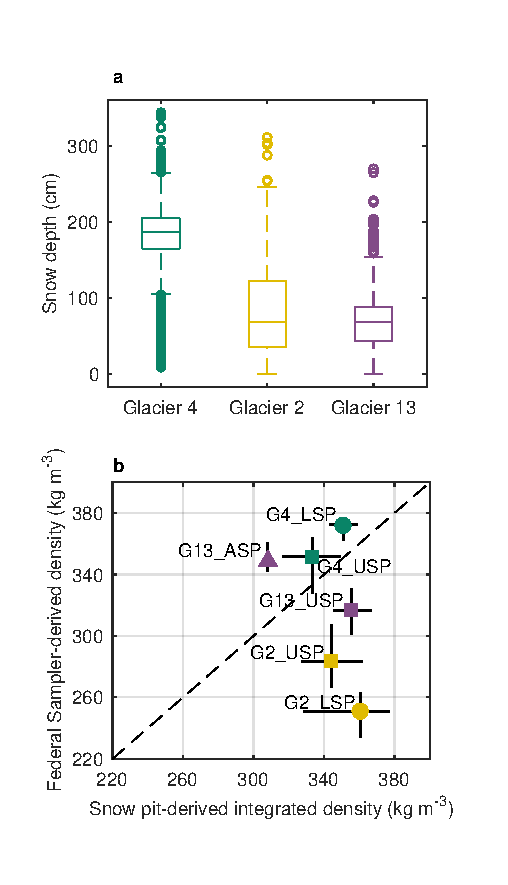
\includegraphics[width =\textwidth]{DepthBoxplot_SPvsFS.pdf}\\
	\caption{(Left) Boxplot of measured snow depth on Glaciers 4, 2 and 13. The box shows first quartiles, the line within the box indicates data median, bars indicate minimum and maximum values (excluding outliers), and circles show outliers, which are defined as being outside of the range of 1.5 times the quartiles (approximately $\pm2.7\sigma$). (Right) Comparison of integrated density estimated using wedge cutters in a snow pit and density estimated using Federal Sampler measurements for Glacier 4 (G04), Glacier 2 (G02) and Glacier 13 (G13). Snow pits were distributed in the accumulation area (ASP), upper ablation area (USP) and lower ablation area (LSP). Error bars are minimum and maximum values.}
	\label{fig:DepthBoxplot_SPvsFS}
\end{figure*}

A wide range of snow depth is observed on all three study glaciers (Figure \ref{fig:DepthBoxplot_SPvsFS}). Glacier 4 has the highest mean snow depth and a high proportion of outliers, indicating a more variable snow depth overall. Glacier 13 has the lowest mean snow depth and a narrower distribution of observed values. At each measurement location, the median range of measured depths ($3-4$ points) as a percent of the mean depth at that location is 2\%, 11\%, and 12\%, for Glaciers 4, 2 and 13, respectively. 

Mean SP and FS density values are within one standard deviation of each other for each glacier and over all three glaciers. The standard deviation of glacier-wide mean density is less than 10\% of the mean density. However, FS densities have a larger range of values ($227-431$kg m$^{-3}$) when compared to SP densities ($299-381$kg m$^{-3}$).  The mean SP densities are within one standard deviation between glaciers, whereas mean FS densities are not.

Uncertainty in SP density is largely due to sampling error of exceptionally dense snow layers. We quantify this uncertainty by varying three values. Ice layer density is varied between 700 and 900 kg m$^{-3}$, ice layer thickness is varied by $\pm$1 cm of the recorded thickness, and the density of layers identified as being too hard to sample (but not ice) is varied between 600 and 700 kg m$^{-3}$. The range of integrated density values is always less than 15\% of the reference density, with the largest ranges present on Glacier 2. Density values for shallow pits that contain ice lenses are particularly sensitive to changes in density and ice lens thickness.

\subsection{Distributed density}

We find no correlation between co-located SP and FS densities (Figure \ref{fig:density_pitVStube}) so each set of density values is used for all four density interpolation options. Regional and glacier mean densities are higher when SP densities are used (Table \ref{tab:Density}). The slope of a linear regression of density with elevation differs between SP and FS densities (Table \ref{tab:Density}). At Glaciers 2 and 13, SP density decreases with elevation, likely indicating melt and/or compaction at lower elevations. SP density is independent of elevation on Glacier 4. FS density increases with elevation on Glacier 2 and there is no relationship with elevation on Glaciers 4 and 13. There is a positive linear relation (R$^2= 0.59$, p$<$0.01) between measured snow density and depth for all FS measurements. No correlation exists between SP density and elevation.

\begin{table}[]
\centering
\caption{Snow density values used for interpolating density based on snow pit (SP) densities and Federal Sampler (FS) densities. Four interpolation methods are chosen: (1) using a mean snow density for all three glaciers (Range mean density), (2) using a mean density for each glacier (Glacier mean density), (3) using a regression between density and elevation (Elevation regression), and (4) inverse-distance weighted mean density (not shown).}
\label{tab:Density}
\begin{tabular}{cccc}
 &  & \textbf{\begin{tabular}[c]{@{}c@{}}SP density\\ (kg m$^{-3}$)\end{tabular}} & \textbf{\begin{tabular}[c]{@{}c@{}}FS density\\ (kg m$^{-3}$)\end{tabular}} \\
 \midrule
\textbf{\begin{tabular}[c]{@{}c@{}}Range \\ mean density\end{tabular}} &  & 342 & 316 \\
\midrule
\multirow{3}{*}{\textbf{\begin{tabular}[c]{@{}c@{}}Glacier\\ mean density\end{tabular}}} & G4 & 348 & 327 \\
 & G2 & 333 & 326 \\
 & G13 & 349 & 307 \\
 \midrule
\multirow{3}{*}{\textbf{\begin{tabular}[c]{@{}c@{}}Elevation \\ regression\end{tabular}}} & G4 & $0.03z+274$ & $-0.16z+714$ \\
 & G2 & $-0.14z+659$ & $0.24z-282$ \\
 & G13 & $-0.20z+802$ & $0.12z+33$
\end{tabular}
\end{table}

\subsection{Grid cell average}

SWE observations within a DEM grid cell are averaged. Between one and six measurement locations are in each measured grid cell. The distribution of grid-cell SWE values for each glacier is similar to that of Figure \ref{fig:DepthBoxplot_SPvsFS} but with fewer outliers. SWE measurements for each zigzag are not normally distributed about the mean SWE (Figure \ref{fig:ZigzagHistogram}). The average standard deviation of all zigzags on Glacier 4 is $\sigma_{\mathrm{G4}} =  0.027$ m w.e., on Glacier 2 is $\sigma_{\mathrm{G2}} =  0.035$ m w.e. and on Glacier 13 is $\sigma_{\mathrm{G13}} =  0.040$ m w.e.

\begin{figure}
	\centering
	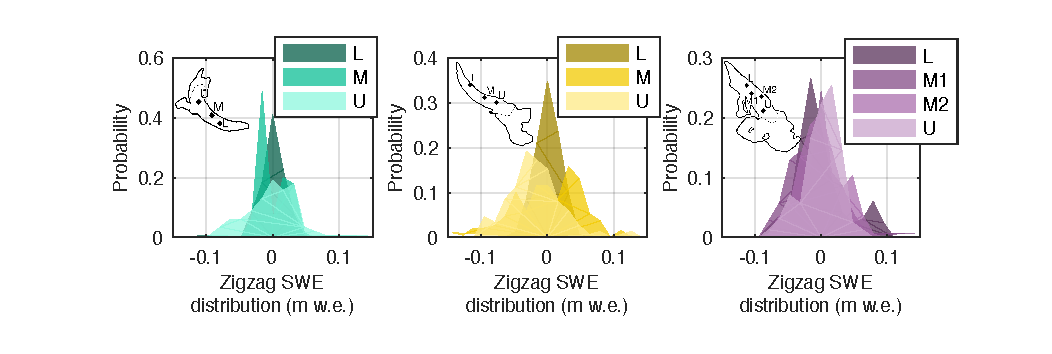
\includegraphics[width =0.5\textwidth]{ZigzagHistogram.pdf}\\
	\caption{Distribution of zigzag SWE values with the local mean subtracted on Glacier 4 (upper panel), Glacier 2 (middle panel) and Glacier 13 (lower panel). Zigzags are distributed throughout the ablation area of each glacier, with one located in the lower portion (L), one in the middle portion (M), and one in the upper portion (U). There were two zigzags in the middle ablation area of Glacier 13.}
	\label{fig:ZigzagHistogram}
\end{figure}

\subsection{Interpolated SWE}
 
The choice of interpolation method affects the specific winter balance (Table \ref{tab:WSMB&RMSE}). SK produces the highest winter balance on Glacier 4 and the lowest winter balance on Glacier 13. winter balance estimated by SK is $\sim$30\% lower than winter balance estimated by LR on Glaciers 2 and 13. When using LR, the winter balance on Glaciers 4 and 2 are similar in magnitude.

The predictive ability of SK and LR differ on the study glaciers. Generally, SK is better able to predict SWE at observed grid cells (Figure \ref{fig:observedVSestimated_S2}) and RMSE for all glaciers is lower for SK estimates (Table \ref{tab:WSMB&RMSE}). Glacier 13 has the lowest RMSE regardless of interpolation method, indicating lower SWE variability. The highest RMSE and the lowest correlation between estimated and observed SWE is seen on Glacier 4 (R$^2=$ 0.12), which emphasizes the highly variable snow distribution. The highest correlation between estimated and observed SWE is on Glacier 2 when SK is used for interpolation (R$^2=$0.84) (Figure \ref{fig:observedVSestimated_S2}). Residuals using LR and SK for all glaciers are normally distributed.

\begin{table}[]
\centering
\caption{Specific winter balance (WB [m w.e.]) estimated using linear regression and simple kriging interpolation for study glaciers. Average root mean squared error (RMSE [m w.e.]) between estimated and observed grid cells for all points, which were randomly selected and excluded from interpolation, is also shown. RMSE as a percent of the WB is shown in brackets.}
\label{tab:WSMB&RMSE}
\begin{tabular}{ccccc}
 & \multicolumn{2}{c}{\textbf{Linear Regression}} & \multicolumn{2}{c}{\textbf{Simple Kriging}} \\
 & WB & RMSE & WB & RMSE \\
  \midrule
\textbf{Glacier 4} & 0.582 & 0.153 (26\%) & 0.616 & 0.134 (22\%) \\
 \midrule
\textbf{Glacier 2} & 0.577 & 0.102 (18\%) & 0.367 & 0.073 (20\%) \\
 \midrule
\textbf{Glacier 13} & 0.381 & 0.080 (21\%) & 0.271 & 0.068 (25\%)
\end{tabular}
\end{table}

\begin{figure*}
	\centering
	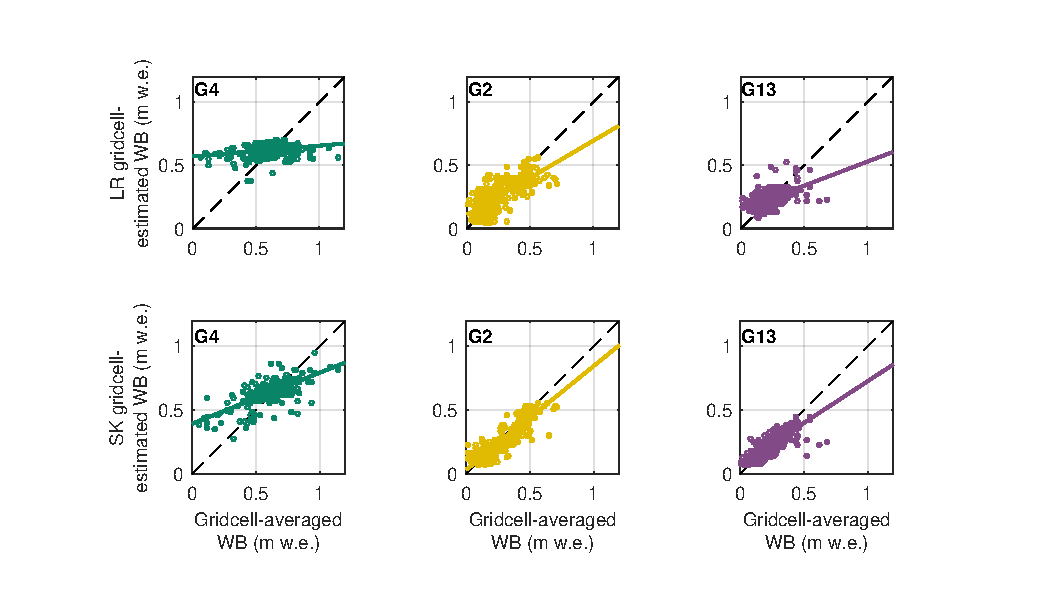
\includegraphics[width =\textwidth]{observedVSestimated_S2.pdf}\\
	\caption{Estimated grid cell SWE found using linear regression (LR) and simple kriging (SK) plotted against observed values of SWE on Glacier 4 (left), Glacier 2 (middle) and Glacier 13 (right). Line of best fit between estimated and observed SWE is also plotted.}
	\label{fig:observedVSestimated_S2}
\end{figure*}

The importance of topographic parameters in the LR differs for the three study glaciers (Figure \ref{fig:BetaCoeffs}). The most important topographic parameter for Glacier 4 is wind redistribution. However, the wind redistribution coefficient is negative, which indicates less snow in `sheltered' areas. Curvature is also a significant predictor of accumulation and the positive correlation indicates that concave areas are more likely to have higher SWE. For Glacier 2, the most important topographic parameter is elevation, which is positively correlated with elevation. Wind redistribution is the second most important topographic parameter and has a positive correlation, which indicates that `sheltered' areas are likely to have high accumulation. The most important topographic parameter for Glacier 13 is elevation. The coefficient is positive, which means that cells at higher elevation have higher SWE. Curvature is also a significant topographic parameter but the correlation is negative, indicating less accumulation in concave areas. Most of the topographic parameters are not significant predictors of accumulation on Glacier 13. Aspect and ``northness'' are not significant predictors of accumulation on all study glaciers.

Our sampling design ensured that the ranges of topographic parameters covered by the measurements represented more than 70\% of the total area of each glacier (except for the elevation range on Glacier 2, which was 50\%). However, we were not able to sample at locations with extreme parameter values and the distribution of the sampled parameters generally differed from the full distribution.


\begin{figure}
	\centering
	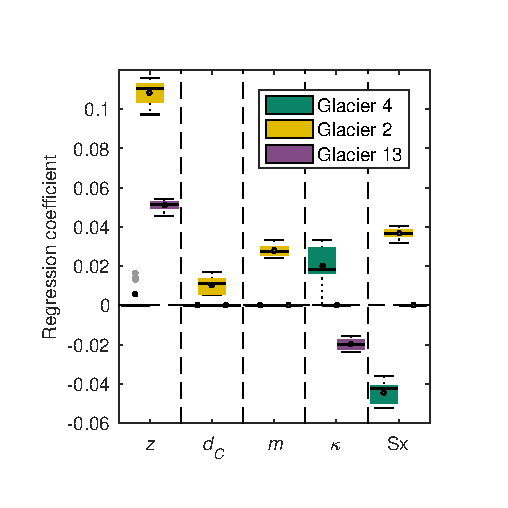
\includegraphics[width =0.5\textwidth]{BetaCoeffs.pdf}\\
	\caption{Distribution of regression coefficients for linear regression of grid cell topographic parameters and SWE calculated using eight density options on study glaciers. Topographic parameters include elevation ($z$), distance from centreline ($d_C$), slope ($m$) , curvature ($\kappa$), and wind exposure (Sx). Regression coefficients that were not significant were assigned a value of zero. Aspect and ``northeness'' are not shown because coefficient values are zero for all glaciers. Outlier values are shown as gray dots.}
	\label{fig:BetaCoeffs}
\end{figure}

Spatial patterns of SWE found using LR are similar between Glaciers 2 and 13 and differ considerably for Glacier 4 (Figure \ref{fig:LR_SK_map}). Estimated SWE on Glacier 4 is relatively uniform, which results from the low predictive ability of the LR. Areas with high wind redistribution values (sheltered), especially in the accumulation area, have the lowest values of SWE. The map of modelled SWE on Glacier 2 closely matches that of elevation, which highlights the strong dependence of SWE on elevation. Glacier 2 has the largest range of estimated SWE ($0 - 1.92$ m w.e). The area of high estimated accumulation in the southwest region of the glacier  results from the combination of high elevation and Sx values. The low SWE values at the terminus arise from low elevation and Sx values close to zero. The map of estimated SWE on Glacier 13 also closely follows elevation. However, the lower correlation between SWE and elevation results in a relatively small range of distributed SWE values.

There are large differences in spatial patterns of estimated winter balance for the three study glaciers found using SK (Figure \ref{fig:LR_SK_map}). On Glacier 4, the isotropic correlation length is considerably shorter (90 m) compared to Glacier 2 (404 m) and Glacier 13 (444 m), which results in a relatively uniform SWE distribution over the glacier with small deviations at measured grid cells. Nugget values for the study glaciers also differ, with the nugget of Glacier 4 (0.0105 m w.e.) more than twice as large as that of Glacier 2 (0.0036 m w.e.) and Glacier 13 (0.0048 m w.e.). Glacier 2 has two distinct and relatively uniform areas of estimated accumulation. The lower ablation area has low SWE ($\sim$0.1 m w.e.) and the upper ablation and accumulation areas have higher SWE values ($\sim$0.6 m w.e.). Glacier 13 does not appear to have any strong patterns and accumulation is generally low ($\sim0.1-0.5$ m w.e.).

SWE estimated with LR and SK differ considerably in the upper accumulation areas of Glaciers 2 and 13. The significant influence of elevation in the LR results in substantially higher SWE values at high elevation, whereas the accumulation area of the SK estimates approximate the mean observed SWE. 

\begin{figure*}
	\centering
	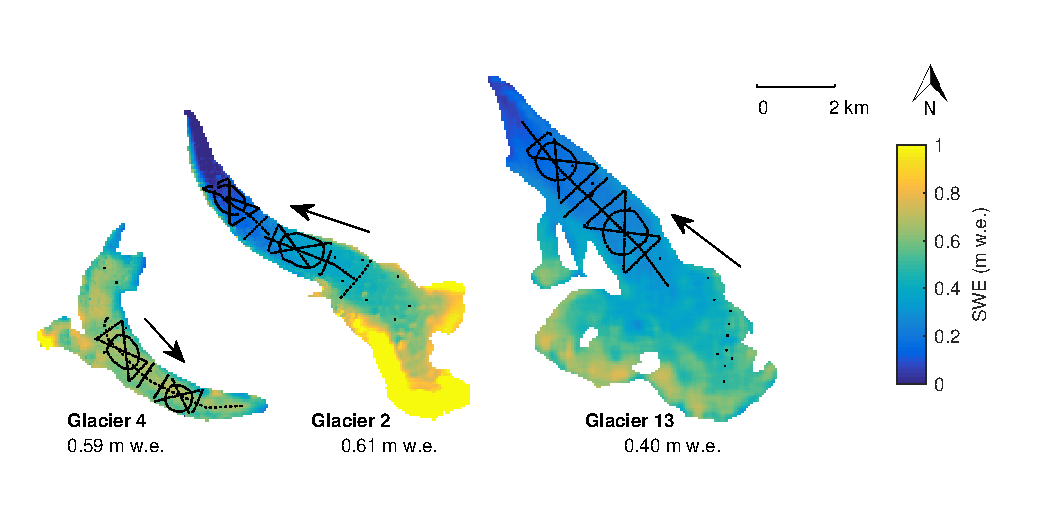
\includegraphics[width =\textwidth]{LR_map.pdf}\\
		\vspace{-16 mm}
    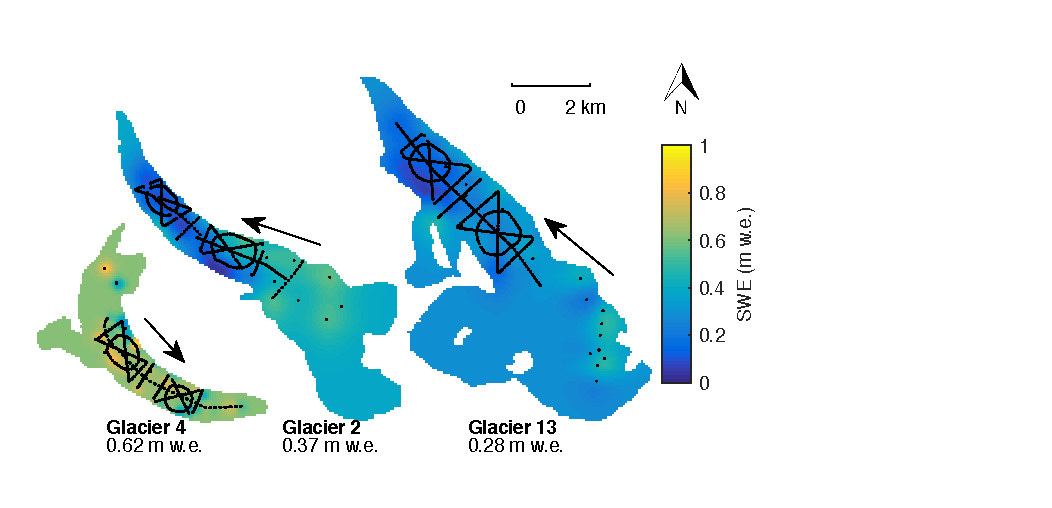
\includegraphics[width =\textwidth]{SK_map.pdf}\\
	\caption{Spatial distribution of SWE estimated using linear regression (upper) and simple kriging (lower). Grid-cell SWE observations are found using glacier wide mean snow pit density and are shown as black dots. Glacier flow directions are indicated by arrows. Specific winter balance values are also shown.}
	\label{fig:LR_SK_map}
\end{figure*}

Transferring LR coefficients between glaciers results in a high RMSE across the mountain range. The lowest overall RMSE (0.2051 m w.e.) results from calculating a LR using all available observations. Elevation is the only significant topographic predictor for a range-scale LR ($\beta_z=0.0525$).

\subsection{Quantifying effects of uncertainty}

Specific winter balance is affected by uncertainty introduced when interpolating density (density uncertainty), when calculating grid cell SWE values (SWE uncertainty), and when interpolating observations (interpolation uncertainty). We find that when using LR and SK, interpolation uncertainty has a larger effect on winter balance uncertainty than density uncertainty or SWE uncertainty. The probability density function (PDF) that arises from SWE uncertainty is much narrower than the PDF that arises from interpolation uncertainty (Figure \ref{fig:WSMBDist_LR} and Table \ref{tab:WSMBdistribution_sigma}).

 \begin{table}[]
\centering
\caption{Standard deviation ([$\times10^{-2}$ m w.e.]) of specific winter balance estimated using linear regression (LR) and simple kriging (SK) when uncertainty is introduced. Density uncertainty ($\sigma_{\rho}$) is the standard deviation of winter balance estimated using SWE data with different density interpolation methods. SWE uncertainty ($\sigma_{\mathrm{SWE}}$) is approximated by a normal distribution about the local SWE value with standard deviation equal to the glacier-wide mean zigzag standard deviation. LR interpolation uncertainty ($\sigma_{INT}$) is accounted for by varying the regression coefficients with a normal distribution with standard deviation calculated from regression covariance. SK interpolation uncertainty ($\sigma_{\mathrm{INT}}$) is taken from the range of distributed SWE estimates calculated by the DiceKriging package. Result for Glacier 4 (G4), Glacier 2 (G2) and Glacier 13 (G13) are shown.}
\label{tab:WSMBdistribution_sigma}
\begin{tabular}{ccccccc}
\textbf{} & \multicolumn{3}{c}{\textbf{Linear Regression}} & \multicolumn{3}{c}{\textbf{Simple Kriging}} \\
 & $\sigma_{\rho}$ & $\sigma_{\mathrm{SWE}}$ & $\sigma_{INT}$ & $\sigma_{\rho}$ & $\sigma_{\mathrm{SWE}}$ & $\sigma_{\mathrm{INT}}$ \\
\midrule
\textbf{G4} & 1.90 & 0.86 & 2.13 & 2.15 & 0.85 & 14.05 \\
\textbf{G2} &3.37 & 1.80 & 3.09 & 2.03 & 2.53 & 13.78 \\
\textbf{G13} & 1.68 & 1.12 & 2.80 & 1.27 & 1.15 & 9.65
\end{tabular}
\end{table}

\begin{figure*}
	\centering
\hspace*{-1.2cm}
	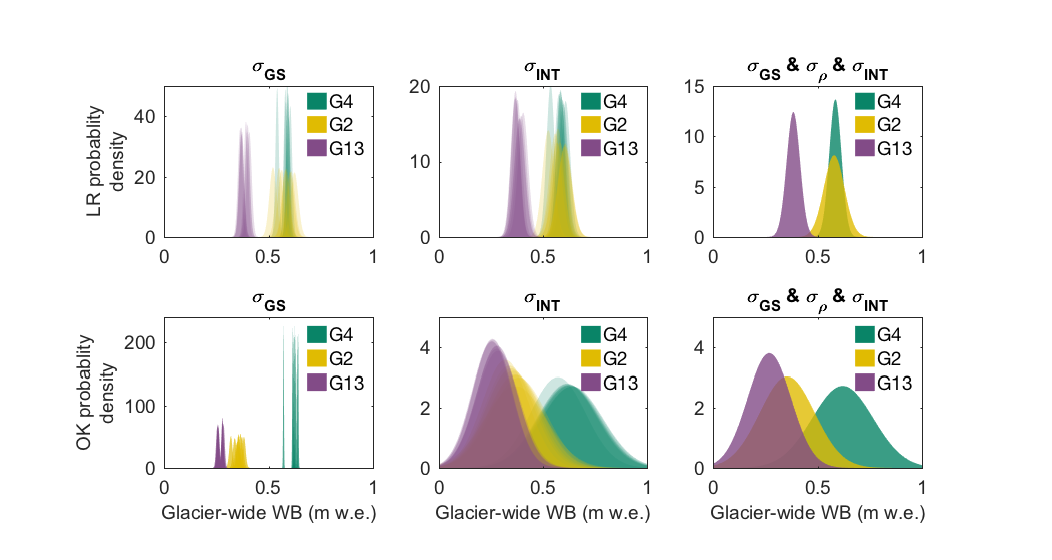
\includegraphics[width =1.2\textwidth]{WSMBDist.pdf}\\
	\caption{Probability density functions (PDFs) fitted to distributions of specific winter balance values that arise from (left) SWE uncertainty ($\sigma_{SWE}$), (middle) interpolation uncertainty ($\sigma_{INTERP}$) and (right) all three sources of uncertainty. Results from a linear regression interpolation (top panels) and simple kriging (bottom panels) are shown. Each PDF is calculated using one of eight density interpolation methods for Glacier 4 (G4), Glacier 2 (G2) and Glacier 13 (G13).}
	\label{fig:WSMBDist_LR}
\end{figure*}

The total winter balance uncertainty from SK interpolation is 3 to 5 times greater than uncertainty from LR interpolation. The PDFs overlap between the two interpolation methods although the PDF modes have lower winter balance values when SK is used for Glaciers 2 and 13 and higher for Glacier 4. SK results in winter balance distributions that overlap between glaciers and there is also a small probability of estimating a winter balance value of 0 m w.e. for Glaciers 2 and 13. LR results in overlapping winter balance distributions for Glaciers 2 and 4, with the PDF peak of Glacier 4 being slightly higher than that of Glacier 2. 

Density, SWE, and interpolation uncertainty all contribute to spatial patterns of winter balance uncertainty (Figure \ref{fig:WSMBspatialvar}).  For both LR and SK, the greatest uncertainty in estimated SWE occurs in the accumulation area. When LR is used, estimated SWE is highly sensitive to the elevation regression parameter. In the case of SK, uncertainty is greatest in areas far from observed SWE, which consist of the upper accumulation area on Glaciers 2 and 13. uncertainty is greatest on Glacier 4 when LR interpolation is used at the upper edges of the accumulation area, which correspond to the locations with extreme values of the wind redistribution parameter. When SK is used for interpolation on Glacier 4, uncertainty is greatest at the measured grid cells, which highlights the short correlation length and the large effect of density interpolation on the SK accumulation estimate.

\begin{figure*}
	\centering
	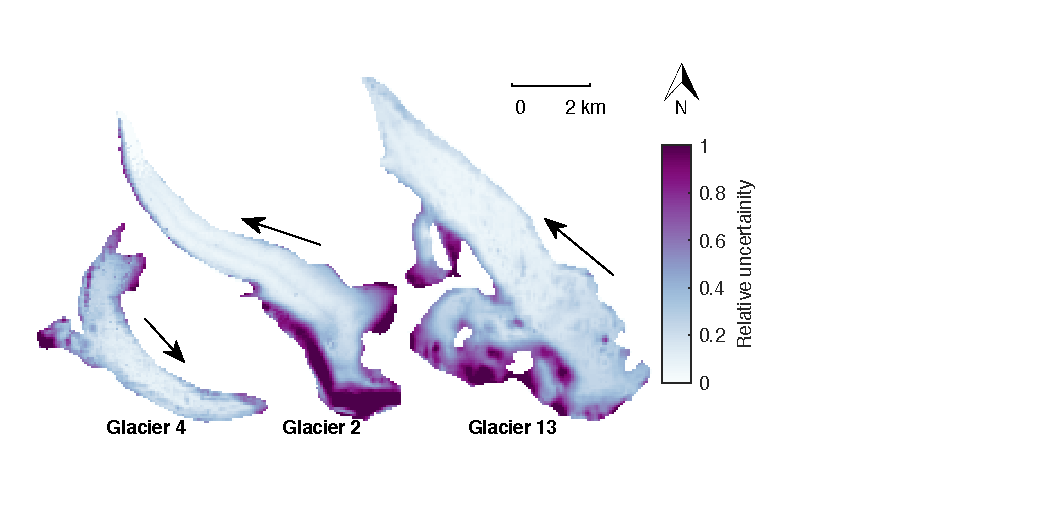
\includegraphics[width =\textwidth]{SpatialVar_LR.pdf}\\
	\vspace{-20 mm}
	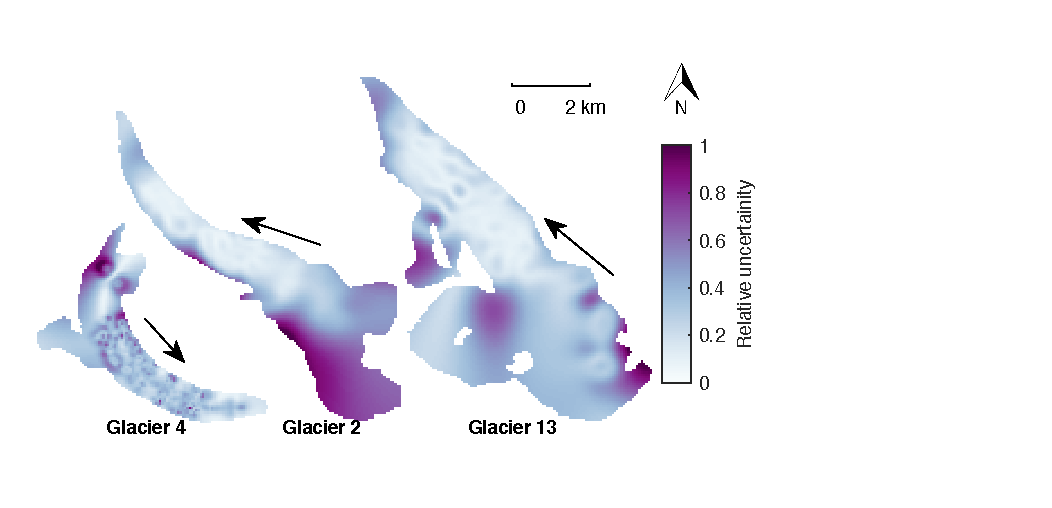
\includegraphics[width =\textwidth]{SpatialVar_SK.pdf}\\
	\caption{Uncertainty of SWE estimated using linear regression (top) and simple kriging (bottom). Uncertainty is a relative quantity measured by taking the sum of differences between one hundred estimates of distributed winter balance that include SWE uncertainty and, in the case of linear regression, regression uncertainty. The sum is then normalized for each glacier. Glacier flow directions are indicated by arrows.}
	\label{fig:WSMBspatialvar}
\end{figure*}



%%%%%%%%%%%%%%%%%%%%%%%%%%%%%%%%%%
% DISCUSSION
%%%%%%%%%%%%%%%%%%%%%%%%%%%%%%%%%%

\section{Discussion}

\subsection{Measurements}

Our study suffers from lack of data in the accumulation area, especially along steep head walls. Snow probing cannot be used reliably in the accumulation area because the snow-firn transition is often difficult to determine. \cite{Sold2013} noted that a systematic bias can result from incorrect values of winter balance, particularly because inaccessible areas such as cliffs and ridges have relatively shallow accumulations (due to wind erosion), while heavily crevassed areas can accumulate deep snow packs. Measuring SWE in the accumulation area is difficult and subject to large errors regardless of the data collection method.

We measured snow density by sampling a snow pit (SP) and by using a Federal Sampler (FS). We found that FS and SP measurements are not correlated and that FS density values are positively correlated with snow depth. This positive relationship could be a result of physical processes, such as compaction, and/or artefacts during data collection. However, it seems more likely that this correlation is a result of measurement artefacts for a number of reasons. First, the range of densities measured by the Federal sampler is large (225--410 kg m$^{-3}$) and the extreme values seem unlikely to exist at these study glaciers at the time of sampling, which experience a continental snow pack with minimal mid-winter melt events. Second, compaction effects would likely be small at these study glaciers because of the relatively shallow snow pack (deepest measurement was 340 cm). Third, no linear relationship exists between depth and SP density (R$^2=$ 0.05). Together, these reasons lead us to conclude that the Federal Sampler measurements are biased but in a way that cannot be easily corrected. 

The FS appears to oversample in deep snow and undersample in shallow snow. Oversampling by small diameter (area of 10--12 cm$^2$) sampling tubes has been observed in previous studies, with a percent error between +6.8\% and 11.8\% \citep{Work1965, Fames1982, Conger2009}. Studies that use Federal Samplers often apply a 10\% correction to all measurements \citep[e.g.][]{Molotch2005}. \cite{Dixon2012} attributed oversampling to slots ``shaving'' snow into the tube as it is rotated as well as cutter design forcing snow into the tube. \cite{Beaumont1963} found that only when snow samples had densities greater than 400 kg m$^{-3}$ and snow depth greater than 1 m, the FS oversampled due to snow falling into the greater area of slots. Undersampling is likely to occur due to snow falling out of the bottom of the sampler \citep{Turcan1975}. It is likely that this occurred during our study since a large portion of the lower elevation snow on both Glaciers 2 and 13 was melt affected and thin, allowing for easier lateral displacement of the snow as the sampler was extracted. For example, on Glacier 13 the snow surface had been affected by radiation melt (especially at lower elevations where the snow was shallower) and the surface would collapse when the sampler was inserted into the snow. It is also difficult to measure the weight of the sampler and snow with the spring scale when there was little snow because the weight was at the lower limit of what could be detected by the scale. Therefore, FS appears to oversample in deep snow due to compaction and/or shaving snow and to undersample in shallow snow due to snow falling out of the sampling tube. 

\subsection{Distributed density}

We choose four different density interpolation methods and separate SP and FS measurements for a total of eight density interpolation options. Despite the wide range of measured density values and different types of density interpolation, density does not appear to strongly affect winter balance estimates and is usually not the dominant source of winter balance uncertainty. Our preferred density interpolation is to use a glacier-wide mean of SP densities. Many winter balance studies assume uniform density \citep[e.g.][]{Elder1991,McGrath2015,Cullen2017} and it is realistic for future studies to measure snow density profiles at a few locations in the study basin. SP measurements are chosen over FS measurements because of the bias observed in FS densities. However, using a glacier-wide mean snow density omits known spatial variability in snow density \citep{Wetlaufer2016}. 

\subsection{Grid cell average}

The zigzag sampling scheme offers a relatively easy way to take a large number of probe measurements in order to capture spatial variability of SWE in a grid cell. While the distribution of SWE values at each zigzag is qualitatively consistent in our study, future studies would benefit from increasing the number of zigzags and focusing on areas with both high variability (e.g. debris covered ice) and low variability (e.g. accumulation area) to determine how variability differs across the glacier.

Since such a large number of points are needed to characterize the variability in a grid cell there is little advantage to measuring and then averaging snow depth at multiple measurement locations. Rather, time should be spent extensively characterizing grid-cell variability in a few locations and to then decrease the spacing of transect measurements to extend their spatial coverage over the glacier. In our study, the grid cell variability appeared to be captured with dense sampling in select grid cells but the basin-scale variability was not captured because sampling was limited to the ablation area. By decreasing transect spacing, grid cells would only have one or two measurements but more grid cells could be measured. 

\subsection{Interpolated SWE}

\subsubsection{Linear regression}

Elevation is the only topographic parameter that offered insight into topographic controls on accumulation. Even so, elevation had little predictive ability for Glacier 4 and the correlation was moderate on Glacier 13. It is possible that the elevation correlation was accentuated, especially on Glacier 13, during the field campaign due to warmer than normal temperatures and an early ($1-2$ weeks) start to the melt season (Yukon Snow Survey Bulletin and Water Supply Forecast, May 1, 2016). The southwestern Yukon winter snow pack in 2015 was also well below average, likely resulting any effects of early melt onset to be emphasized.

Elevation affects snow distribution through melt at lower elevation due to higher temperatures, as well as increased precipitation and preservation of snow at higher elevation. Glacier 4 had deeper snow and cloudier conditions during the field campaign so perhaps a correlation between SWE and elevation had not manifested itself. 

Our mixed insights into dominant predictors of accumulation are consistent with the conflicting results present in the literature. Many winter balance studies have found elevation to be the most significant predictor of SWE \citep[e.g.][]{Machguth2006, McGrath2015}. However, accumulation-elevation gradients vary considerably between glaciers \citep{Winther1998} and other factors, such as orientation relative to dominant wind direction and glacier shape, have been noted to affect accumulation distribution \citep{Machguth2006,Grabiec2011}.  \cite{Machguth2006}, \cite{Grunewald2014} and \cite{Kirchner2014} observed elevation trends in snow accumulation for the lower parts of their study basins but no correlation or even a decrease in SWE with elevation for the upper portion of their basins. \cite{Helbig2017} suggest that an increase in accumulation with elevation can better be approximated by a power law (of the form $y=ax^k$ with $k\>1$). There are also a number of accumulation studies on glaciers that found no significant correlation between accumulation and topographic parameters and the highly variable snow distribution was attributed to complex local conditions \citep[e.g.][]{Grabiec2011,Lopez2011}.

Wind redistribution and preferential deposition of snow is known to have a large influence on accumulation at sub-basin scales\citep{Dadic2010, Winstral2013}. The wind redistribution parameter used in our study is found to be a small but significant predictor of accumulation on Glacier 4 (negative correlation) and Glacier 2 (positive correlation). This result indicates that wind likely has an impact on snow distribution but that the wind redistribution parameter is perhaps not the most appropriate way to characterize the effect of wind on our study glaciers. For example, Glacier 4 is located in a curved valley with steep side walls so having a single cardinal direction for wind may be inappropriate. Examining wind redistribution parameter values that assume wind moving up or down glacier and changing direction to follow the valley could allow the wind redistribution parameter to explain more of the variance in SWE. Additionally, sublimation from blowing snow has been shown to be an important mass loss from ridges \citep{Musselman2015}. Incorporating snow loss as well as redistribution and preferential deposition may be needed for accurate representations of seasonal accumulation. Further, the scale of deposition may be smaller than the resolution of the Sx parameter in the relatively large DEM grid cells in our study. An investigation of the wind redistribution parameter with finer DEM resolution is also needed. A universal predictor of distributed SWE therefore continues to elude researchers and accumulation variability due to complex interactions between topography and the atmosphere needs to be considered when estimating winter mass balance. 

Since we were unable to measure SWE in grid cells that have high topographic parameter values, we must extrapolate relationships linearly. The accumulation area, where there are few observations, is most susceptible to extrapolation errors. This area typically also has the highest SWE values, affecting the specific winter balance estimated for the glacier. In our study, the dependence of SWE on elevation, especially on Glacier 2, means that LR extrapolation results in almost 2 m w.e. estimated in the parts of the accumulation area. This exceptionally large estimate of SWE is unlikely for a continental snow pack. Extrapolating a LR that is fitted to predominantly ablation area SWE values is likely erroneous. 

While a LR can be used to predict distributed SWE in other basins, we found that transfer of LR coefficients between glaciers results in large estimation error. Applying LR coefficients to unmeasured basins therefore results in high winter balance uncertainty. The LR fitted to all observed data produced the best overall predictor of SWE in the Donjek Range. Our results are consistent with \cite{Grunewald2013}, who found that local statistical models are able to perform well but  they cannot be transferred to different regions and that regional-scale models are not able to explain variance. The inter-basin variability in our study range is greater than the intra-basin variability. 

\subsubsection{Simple kriging}

For all study glaciers, simple kriging (SK) is a better predictor of observed SWE than LR. However, the winter balance uncertainty that arises from using SK is large, and unrealistic values of 0 m w.e. winter balance can be estimated. Our observations are generally limited to the ablation area so SK estimates an almost uniform distribution of SWE in the accumulation areas of the study glaciers, which is inconsistent with observations described in the literature. Extrapolation using SK leads to large uncertainty in estimating winter balance, which further emphasis the need for SWE observations in the accumulation area. 

SK cannot be used to understand physical processes that may be controlling snow distribution and cannot be used to estimate accumulation beyond the study area. However, fitted kriging parameters, including the nugget and spatial correlation length, can provide insight into important scales of variability. Glaciers 2 and 13 have long correlation lengths and small nuggets indicating variability at large scales. Conversely, Glacier 4 has a short correlation length and large nugget, indicating that accumulation variability occurs at small scales. Using a higher resolution sampling design and DEM may allow us to capture more of the variability on Glacier 4 and to perhaps improve the predictive ability of both LR and SK interpolation. 

A number of studies that relate SWE to topographic parameters have found success when using a regression tree interpolation model, which is a non-linear regression method \citep[e.g.][]{Elder1998, Erickson2005, Lopez2010}. Many relationships between accumulation and topographic parameters have been observed to be non-linear so regression tree are valuable in snow modelling and may yield improved results \citep{Erxleben2002, Molotch2005}. 

\subsection{Quantifying effects of variability}

%Interpolation uncertainty is the greatest contributor to winter balance uncertainty for both SK and LR. A large contributor to uncertainty arises from extrapolation beyond the sampled region, which results in high uncertainty in estimated SWE in the accumulation area. 

SWE uncertainty is the smallest contributor to winter balance uncertainty. Therefore, obtaining the most accurate value of SWE to represent a grid cell, even a relatively large grid cell, does not need to be a priority when designing a snow survey. Many parts of a glacier are characterized by a relatively smooth surface, with roughness lengths on the order of centimeters \citep{Hock2005} resulting in low snow depth uncertainty. However, we assume that the sampled grid cells are representative of the uncertainty across the entire glacier, which is likely not true for areas with debris cover, crevasses and steep slopes. 

Using a Monte Carlo experiment to propagate uncertainty allowed us to quantify effects of uncertainty on estimates of winter balance. However, our analysis did not include uncertainty arising from a number of data sources, which we assumed to contribute negligibly to the uncertainty in winter balance. These sources of uncertainty include error associated with SP and FS density measurement, DEM vertical and horizontal error and error associated with estimating measurement locations.

\subsection{Mountain range accumulation gradient}

An accumulation gradient is observed for the continental side of the St. Elias Mountains (Figure \ref{fig:AccumGrad}). Accumulation data are compiled from \cite{Taylor1969}, the three glaciers presented in this paper, as well as two snow pits we dug near the head of the Kaskawalsh Glacier in May 2016. The data show a linear decrease in observed SWE as distance from the main mountain divide (identified by \cite{Taylor1969}) increases, with a gradient of $-0.024$ m w.e. km$^{-1}$. While the three study glaciers fit the regional relationship, the same relationship would not apply when just the Donjek Range is considered. Therefore, glacier location within a mountain range also affects glacier-wide winter balance. Interaction between meso-scale weather patterns and mountain topography is a major driver of glacier-wide accumulation. Further insight into mountain-scale accumulation trends can be achieved by investigating moisture source trajectories and orographic precipitation contribution to accumulation. 

\begin{figure}
	\centering
	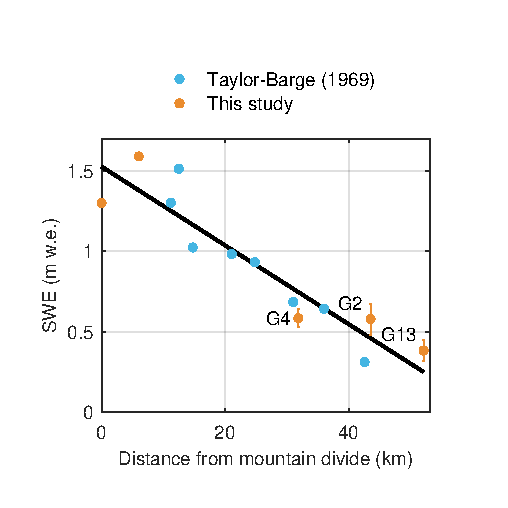
\includegraphics[width =0.5\textwidth]{AccumGrad.pdf}\\
	\caption{Relation between SWE and linear distance from St. Elias mountain divide, located at the head of the Kaskawalsh Glacier. Blue dots are snow pit derived SWE values from \cite{Taylor1969}. Orange dots furthest from the divide are mean winter balance from Glaciers 4, 2 and 13, with 95\% confidence interval using a linear regression interpolation. Orange dots close to the divide are snow pit derived SWE value at two locations in the accumulation area of the Kaskawalsh Glacier collect in May 2016. Black line indicates line of best fit (R$^2=0.85$).}
	\label{fig:AccumGrad}
\end{figure}


\subsection{Limitations and future work}

Extensions to this work could include an investigation of experimental design, examining the effects of DEM grid size on winter balance and resolving temporal variability. 

Our sampling design was chosen to extensively sample the ablation area and is likely too finely resolved for many future mass balance surveys to replicate. Determining a sampling design that minimizes error and reduces the number of measurements, known as data efficiency thresholds, would contribute to optimizing snow surveys in mountainous regions. For example, \cite{Lopez2010} concluded that $200-400$ observations are needed to obtain accurate and robust snow distribution models. 

DEM grid cell size is known to significantly affect computed topographic parameters and the ability for a DEM to resolve important hydrological features (i.e. drainage pathways) in the landscape \citep{Zhang1994, Garbrecht1994, Guo-an2001, Lopez2010}, which can have implications for calculating a LR for SWE data.  \cite{Zhang1994} found that a 10-m grid cell size is an optimal compromise between increasing resolution and large data volumes. Further, the importance of topographic parameters in predicting SWE is correlated with DEM grid size \citep[e.g.][]{Kienzle2004, Lopez2010}. A decrease in spatial resolution of the DEM resulted in a decrease in the importance of curvature and an increase in the importance of elevation. A detailed and ground controlled DEM is therefore needed to identify the features that drive accumulation variability. Future studies could also evaluate the effects of DEM uncertainty on elevation and derived topographic parameters \citep [e.g.][]{Guo-an2001, Wechsler2006}.

Temporal variability in accumulation is not considered in our study. While this limits the extent of our conclusions, a number of studies have found temporal stability in spatial patterns of snow accumulation and that terrain-based model could be applied reliable between years \citep[e.g.][]{Grunewald2013}. For example, \cite{Walmsley2015} analysed more than 40 years of accumulation recorded on two Norwegian glaciers and found that snow accumulation is spatially heterogeneous yet exhibits robust time stability in its distribution. 

%%%%%%%%%%%%%%%%%%%%%%%%%%%%%%%%%%
% CONCLUSION
%%%%%%%%%%%%%%%%%%%%%%%%%%%%%%%%%%
\section{Conclusion}

We estimate spatial accumulation patterns and specific winter balance for three glaciers in the St. Elias mountains from extensive snow depth and density sampling. Our objectives are to (1) examine methods and uncertainties when moving from snow measurements to estimating winter balance and (2) show how snow variability, data error and our methodological choices interact to create uncertainty in our estimate of winter balance.

Overall, elevation is the dominant driver of SWE distribution but results vary between glaciers. Accumulation spatial patterns and scales of variability are considerably different on Glacier 4 when compared to Glaciers 2 and 13. Glaciers 2 and 13 have a dominant elevation-accumulation trend and long spatial correlation lengths. No topographic parameters were able to explain snow distribution on Glacier 4 and a short correlation length and large nugget indicate variability at shorter length scales. Our results also suggest that wind redistribution and preferential distribution are significant drivers of SWE distribution but these effects are not captured by the wind redistribution parameter used. Improved modelling of wind effects on accumulation through modification of the wind redistribution parameter as well as increased physical modelling are needed. A LR applied to our study glaciers resulted in little insight into dominant physical processes indicating that accumulation is controlled by complex interactions between topography and the atmosphere and that a finer resolution DEM is needed to resolve SWE distribution and potentially relevant topographic parameters, such as curvature and wind redistribution.

Glacier accumulation is strongly affected by interactions between topography and atmospheric processes at the basin- and range-scale. Although we could not conclusively identify processes at the basin scale due to low predictive ability of the LRs, there is a dominant trend in accumulation at the range scale. We identify a clear linear decrease in SWE with increased distance from the main topographic divide along the continental side of the St. Elias Mountains. This trend indicates that glacier location within a mountain range has a large influence on winter balance. Further investigation of meso-scale weather patterns could provide insight into relevant processes that affect accumulation at the range scale.

We also quantify the effects of variability from density interpolation, grid cell SWE calculation as well as interpolation method on uncertainty in estimating winter balance. We conduct a Monte Carlo experiment to propagate variability through the process of estimating accumulation from snow measurements. The largest source of uncertainty in our study stems from variability in interpolation method, both within and between methods. We find that SK results in high uncertainty and the distribution of winter balance estimates  encompasses unrealistic values. Spatial distribution of interpolation variability indicates that the accumulation area is the greatest area of uncertainty. This large variability is a result of the accumulation area being poorly sampled, sensitive to estimates of dominant regression coefficients, and having the largest values of estimated SWE within the glacier. To better constrain winter balance estimates, future studies should focus on obtaining snow measurements in the accumulation area at the expense of collecting less data overall. Density and SWE variability are found to be small contributors to winter balance uncertainty. We conclude that the choice of interpolation method in combination with sampling design, especially in the accumulation area, has a major impact on the uncertainty in winter balance estimates.



%----------------------------------------------------------------------------------------
%	REFERENCE LIST
%----------------------------------------------------------------------------------------
%
\bibliography{/home/glaciology1/Documents/MastersDocuments/MastersLit}
%\bibliography{/Users/Alexandra/Documents/SFU/MastersDocuments/MastersLit}
\bibliographystyle{igs}

%----------------------------------------------------------------------------------------

%
%%1
%Snow distribution affects the availability of water for human and ecological needs. In alpine regions, glaciers act as important mediators of this relationship by delaying snow melt and providing water from ice melt during the late summer. The distribution of snow on glaciers therefore has a large impact on water resources. Snow is also the dominant input of glacier mass and decreasing uncertainty in estimating winter mass balance by focusing on the  amount and spatial distribution of winter accumulation is central to assessing health of glaciers \citep{Reveillet2016}. Glacier mass loss is predicted to contribute ?? m to global sea level rise so understanding how local glacier mass balance is affected by distribution of snow is critical for accurate predictions of glacier response to a warming climate. Snow distribution is sensitive to a number of complex process that partially depend on glacier location, topography, and orientation. Current models are not able to fully represent these processes so the distribution of snow in remote, mountainous locations is not well known. This is a significant source of uncertainty that undermines the ability of models to represent current glacier conditions and make predictions about how they will change.
%
%%2
%Snow distribution in alpine regions is not uniform or static, but rather highly variable and influenced by diverse and dynamic interactions the atmosphere and complex topography operating on multiple spatial and temporal scales. Several key processes are responsible for patterns of snow distribution. Orographic precipitation associated with air mass lifting along high topographic slopes generally results in increased precipitation at higher elevations \citep{Clark2011, Sold2013}. Cooler temperatures at high elevations result in more precipitation falling as snow, further increasing the amount of snow at high elevation \citep{Bloschl1991}. Location of a basin within a mountain range and its proximity to a moisture source also affects the overall amount of snow \citep{McGrath2015}. Decreased precipitation is observed on the lee side of topographic divides and in locations further from large bodies of water. Solar radiation causes increased snow melt on south-facing slopes \citep{Mott2008}. Wind redistribution and preferential deposition are crucial factors that influence the distribution of snow \citep{Lehning2008, Winstral2002, Clark2011}. Sharp changes in topography cause convergent and divergent airflows close to the surface, leading to terrain induced turbulence that modifies mean wind and snow particle velocities \citep{Mott2008, Lehning2008, Dadic2010}. In general, high wind speeds and up drafts on the windward side of ridges causes reduced deposition and increased erosion of snow. On the leeward side of a ridge, lower wind speeds result in snow particle fall out and deposition leading to increased accumulation \citep{Liston1998, Mott2011}. 
%
%The atmospheric processes interact with complex mountain topography to create variability in snow distribution at multiple spatial scales. \cite{Clark2011} identifies the point scale ($<$5 m), hillslope scale (1--100 m), basin scale (100--10,000 m) and regional scale (10--1000 km) as the most important scales for snow accumulation. Topographic features on glaciers and surrounding mountains such a rocks, crevasses, local ridges and depressions and variations in curvature and slope can affect where snow is located  \citep{Bloeschl1999, Sold2013}. Avalanching can also redistribute snow, especially on the margins of a glacier \citep{Bloschl1991, Mott2008}. 
%
%%3
%Estimating the distribution and variability of snow accumulation requires accurately accounting for the interaction of atmospheric processes and topography. Dynamic models use known physical relationships to simulate temporally and spatially resolved surface processes and use the results to predict where and how much snow will be deposited \citep{Mott2008}. Dynamic models are a valuable way to determine accumulation variability but application is operationally complex and computationally expensive, and also requires a diverse set of detailed observations. Statistical models of snow variability establish empirical relationships between snow distribution and external variables, which act as proximes for physical processes \citep{Fowler2007}. Two commonly applied statistical techniques that interpolate and extrapolate snow measurements include regression and kriging. 
%
%Measuring snow can be done in a number of 
%
%
%%5
%The St. Elias Mountains contain the largest non-polar ice field and the longest valley glaciers outside of Greenland and Antarctica \citep{Marcus1970, Marcus1970}. Steep climatic gradients across the mountains create sharp changes in glacier cover and mass balance \citep{Clarke2002}. This region currently has the most negative mass budget and is the largest contributor to sea-level rise in the world \citep{Kaser2006,Gardner2013}. Research on snow distribution and glacier mass balance in the St. Elias is limited. The first significant investigations took place under Project Snow Cornice \citep{Wood1948}. Researchers looked at snow accumulation and ice formation as well as ice-mass thermal regime, density, and depth. Studies were conducted primarily on large glaciers such as the Kaskawalsh and Seward, and thus provided insights into large-scale accumulation patterns. This initiative was then followed by the Icefield Ranges Research Project (IRRP), which was established in 1961 \citep{Danby2003}. A number of subsequent long-term studies have been established in the St. Elias since IRRP \citep[e.g.][]{Clarke1984, Paoli2009}. \cite{Arendt2008} and \cite{Wheler2014} briefly studied the mass balance of a number of glaciers throughout the St. Elias. Ice cores have also been used to study the local and regional climate and precipitation history \citep{Holdsworth1991, Moore2002, Wake2002}. 
%
%The weather in the St. Elias varies considerably over the range. The west side of the mountains is characterized by a cool, Marine West Coast climate due to the influence of the Pacific ocean, while the eastern side (just 250 from the ocean) is considered subarctic \citep{Marcus1970}. The mountains are oriented perpendicular to frequent and intense storms that originate in the ocean, which are orographically lifted resulting in significant precipitation \citep{Taylor1969}. Eventually, the fronts spill over the mountain divide (located to the west of the Kaskawalsh Glacier) and descend along the eastern side, which often results in decreased precipitation. This rain shadow is likely the major cause of the significant difference in accumulation and equilibrium line altitude (ELA) between the two sides of the mountains. The marine side has an ELA of $\sim$1100 m and the continental side has an ELA of $\sim$2100 m, while at the same elevation there is three times more accumulation on the marine side \citep{Marcus1970}.
%
%There is clearly a strong need for a more comprehensive understanding of snow accumulation in the St. Elias Mountains. Although a few studies have examined accumulation, no studies have examined the distribution of snow and how it varies spatially, especially on small alpine glaciers. 
%
%%6
%The main objectives of our study are to (1) conduct a comprehensive sweep of choices and assumptions made when moving from snow measurements to estimating accumulation and (2) show how snow variability, data error and our methodological choices interact to create uncertainty in our estimate of accumulation. 

\end{document}
